\chapter{Resultats}

  Per tal de comprovar si el sistema funcionava, s'ha provat de fer un joc senzill amb ell, en aquest cas, un clon del Tetris. En aquest capítol farem un resum del seu desenvolupament i en mirarem el rendiment. Se'n pot veure una captura a la figura \ref{fig:ImatgeTetris}.

  \begin{figure}
    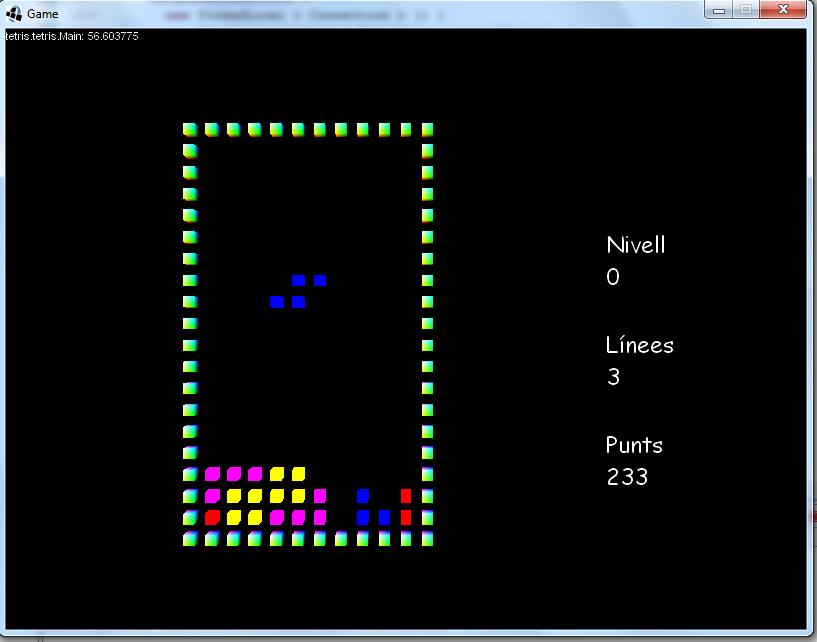
\includegraphics[width=1\linewidth]{./img/ImatgeTetris.png}
    \caption{Captura de pantalla del joc final \label{fig:ImatgeTetris}}
  \end{figure}

\section{Estructura del Tetris en Quadriga}

  Per tal de veure visualment com està muntat aquest tetris, s'ha fet un diagrama semblant a l'UML de la seva estructura a la figura \ref{fig:TetrisEntitats}. També s'ha confeccionat una llegenda per entendre-ho millor que es pot veure a la figura \ref{fig:GuiaDiagramaQuadriga}.

  \begin{figure}
    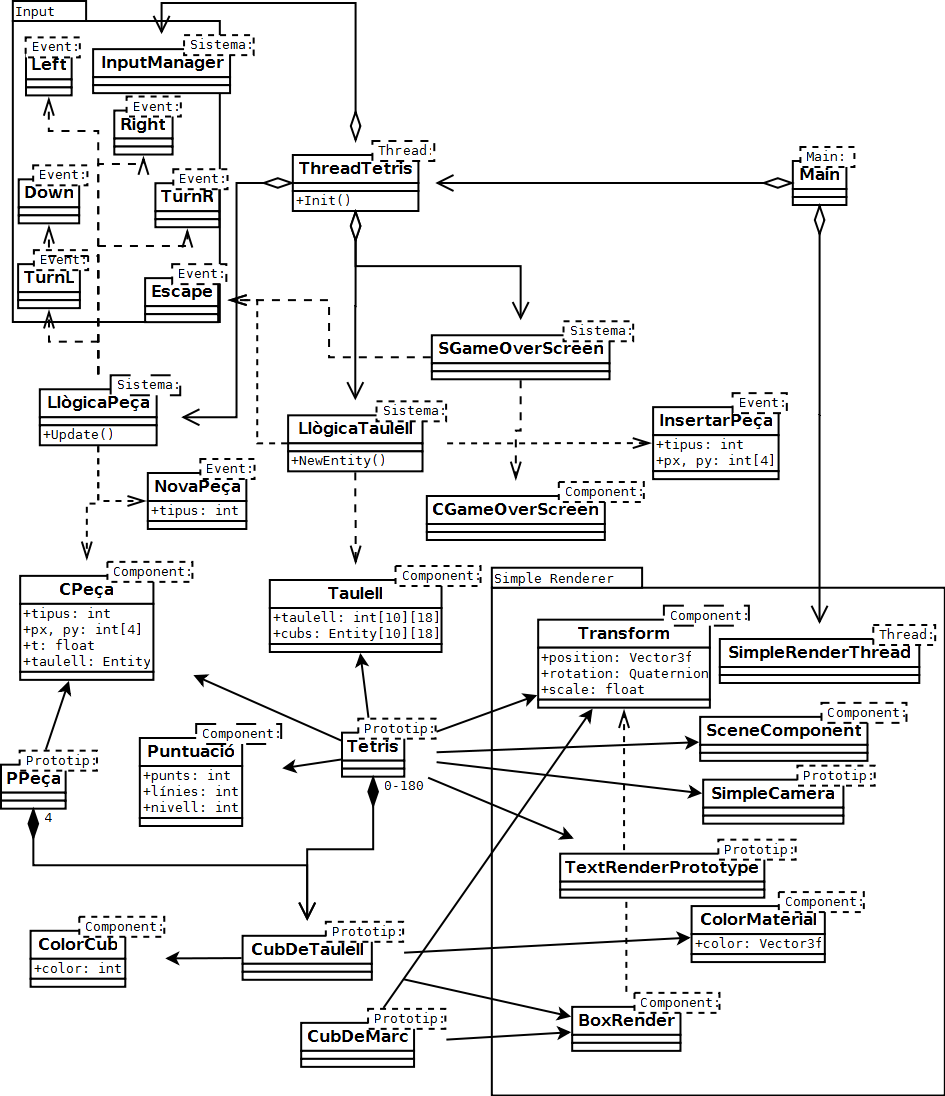
\includegraphics[width=1\linewidth]{./img/TetrisEntitats.png}
    \caption{Esquema dels elements que formen el tetis \label{fig:TetrisEntitats}}
  \end{figure}

  \begin{figure}
    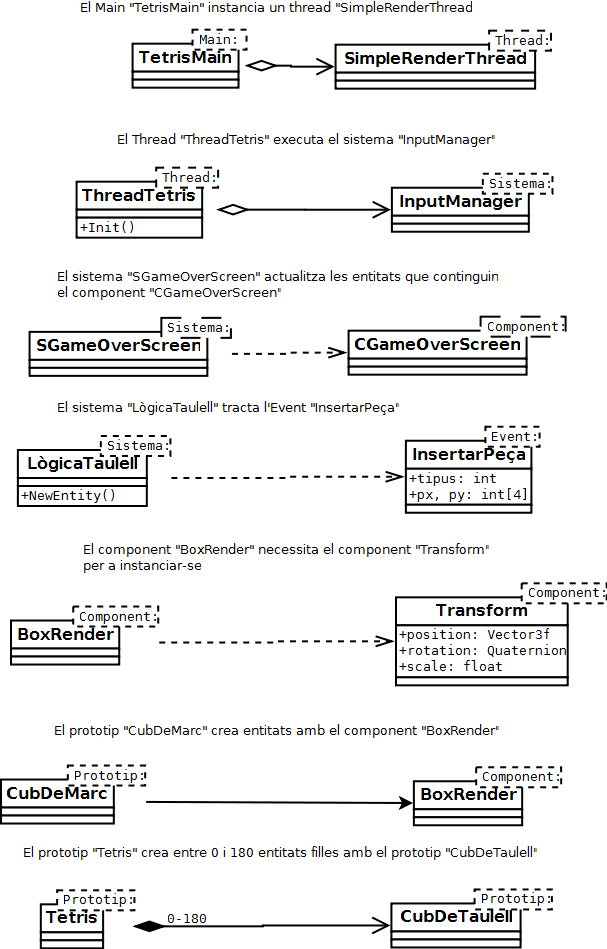
\includegraphics[width=1\linewidth]{./img/GuiaDiagramaQuadriga.png}
    \caption{Llegenda \label{fig:GuiaDiagramaQuadriga}}
  \end{figure}

  \subsection{Elements propis del Tetris}

    \subsubsection{Entitats / Prototips}

      \begin{itemize}
        \item {\bf Tetris}
          Representa l'estat actual del taulell de joc, amb els cubs posats, així com també conté informació sobre el nivell actual, els punts i les línies aconseguides per el jugador.
          
        \item {\bf Peça}
          Representa la peça que el jugador ha de col·locar en cada moment. Seria el més semblant a l'Avatar del jugador.
          
        \item {\bf CubDeMarc}
          Representa cada un dels cubs que fan de marc del taulell de joc.
          
        \item {\bf CubDeTaulell}
          Representen els cubs interiors del taulell, tant els col·locats com els que la peça actual aporta. Es diferencien dels anteriors ja que aquests han de tenir un color diferent depenent de la peça.
          
      \end{itemize}

    \subsubsection{Components}

      \begin{itemize}
        \item {\bf Taulell}
          Guarda informació de quines caselles del taulell estan ocupades per un cub, i en guarda una referència per eliminar-los o moure'ls quan el jugador completa una línia.
          
        \item {\bf Puntuació}
          Guarda informació sobre el nivell, les línies completades i la puntuació feta.
          
        \item {\bf Peça}
          Guarda informació sobre la forma i posició de la peça que actualment cau.
          
        \item {\bf ColorCub}
          Guarda informació sobre el color d'un cub.
          
        \item {\bf GameOverScreen}
          Representa la pantalla final, quan el jugador s'ha rendit o ha perdut.
          
      \end{itemize}

    \subsubsection{Events}

      \begin{itemize}
        \item {\bf NovaPeça}
          Es crea una nova peça, ja sigui per que s'inicia el joc o s'ha col·locat l'anterior. Aporta informació sobre quin tipus de peça s'ha de crear.
          
        \item {\bf InserirPeça}
          La peça ha arribat a sota i s'ha d'inserir al taulell.
          
        \item {\bf Left, Right, Down, TurnL, TurnR}
          El jugador ha donat instruccions per moure la peça o girar-la.
          
        \item {\bf Escape}
          El jugador ha premut la tecla d'escapament, volent finalitzar el joc o programa.
          
      \end{itemize}

    \subsubsection{Sistemes}

      \begin{itemize}
        \item {\bf LlògicaTaulell}
          Controla la inserció de peces, l'acumulació de punts i si s'han completat línies, augmentant el nivell si s'escau.
          
        \item {\bf LlògicaPeça}
          Controla que una peça es mogui segons les ordres del jugador i caigui a una velocitat donada per el nivell actual. També comprova si ha arribat al final i cal inserir-la.
          
        \item {\bf GameOverScreen}
          Un cop el jugador ha acabat la partida, en mostra la puntuació i espera que el jugador doni ordres de tancar el programa.
          
        \item {\bf InputManager}
          Vigila quin input dona el jugador i crea els events corresponents.
          
      \end{itemize}
      
    \subsubsection{Threads}
    
      \begin{itemize}
        \item {\bf ThreadTetris}
          Inicialitza el joc i executa els 4 sistemes anteriors.
          
      \end{itemize}
    
  \subsection{Llibreria SimpleRender}

    \subsubsection{Entitats / Prototips}

      \begin{itemize}
        \item {\bf TextRenderer}
          Renderitza un text donada una {\em Font}, una posició i un {\em String}.
      \end{itemize}


    \subsubsection{Components}

      \begin{itemize}
        \item {\bf Transform}
          Guarda informació sobre la translació, rotació i escala d'una entitat.
          
        \item {\bf SceneComponent}
          Marca un objecte com a arrel de l'escena.
          
        \item {\bf SimpleCamera}
          Guarda informació sobre la càmera de l'escena.
          
        \item {\bf ColorMaterial}
          L'objecte es renderitza amb un material de color pla.
          
        \item {\bf BoxRender}
          L'objecte es renderitza com una caixa.
          
      \end{itemize}
      
    \subsubsection{Threads}
    
      \begin{itemize}
        \item {\bf SimpleRenderThread}
          Renderitza tots els objectes de l'escena que contenen algun component \"{}renderitzable\"{} com {\em BoxRender}.
          
      \end{itemize}
      
\section{Objectius de disseny}

  Analitzem, punt per punt, si s'han complert els objectius de disseny del programa.

  \begin{description}
    \item[Open Source] \hfill \\
      El codi es pot trobar a \url{https://code.google.com/p/quadriga/} sota llicència {\bf GNU Lesser GPL}.
      
    \item[El sistema d'entitats ha de ser independent] \hfill \\
      En l'exemple s'usen unes quantes llibreries Java per implementar aspectes importants del joc. {\em OpenGL} i el {\em input} del jugador s'obtenen a partir de {\bf LWJGL}. Per fer-les servir des de {\em Quadriga} cal emprar {\em Components} que anomenaríem "estàndard" sota el paquet {\em cat.quadriga.base}. Fer aquests components no és senzill, però es podrien substituir els sistemes si es volgués fer l'esforç sense masses problemes.
      
    \item[Ha de ser multi-plataforma de forma nativa] \hfill \\
      Com es veu a la figura \ref{fig:ImatgeUbuntu}, el joc corre sobre {\em Ubuntu} sense cap diferència. El codi Java i Quadriga no s'han tocat, però si que cal fer una petita modificació a l'hora de crear l'executable, doncs {\em OpenGL} necessita accedir a llibreries natives que són diferents en cada plataforma.
      
    \item[Ha de permetre un desenvolupament ràpid un cop estiguin fets els components bàsics] \hfill \\
      El codi final són 2 arxius, un de lògica de unes 800 línies i un altre de input de 65. És de fet quasi més llarg fer el disseny que no implementar-lo.
      
    \item[Ha de ser fàcilment paral·lelitzable] \hfill \\
      Actualment el programa conté una opció de fer córrer cada {\em Thread} en paral·lel, però la opció teòricament òptima de paral·lelitzar l'actualització de cada entitat sobre cada sistema (aconseguint una paral·lelització no sobre el nombre de threads, sinó sobre el nombre d'entitats) no s'ha implementat.
  \end{description}
    
  \begin{figure}
    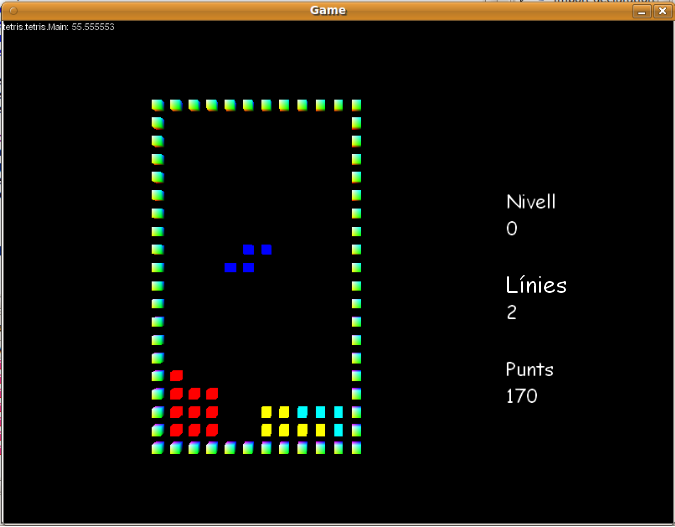
\includegraphics[width=1\linewidth]{./img/ImatgeUbuntu.png}
    \caption{Captura de pantalla del joc sobre Ubuntu \label{fig:ImatgeUbuntu}}
  \end{figure}